\documentclass{standalone}
\usepackage{tikz}
\usepackage{ctex,siunitx}
\usepackage{tkz-euclide}
\usepackage{amsmath}
\usetikzlibrary{patterns, calc}
\usetikzlibrary {decorations.pathmorphing, decorations.pathreplacing, decorations.shapes,}
\begin{document}
\small
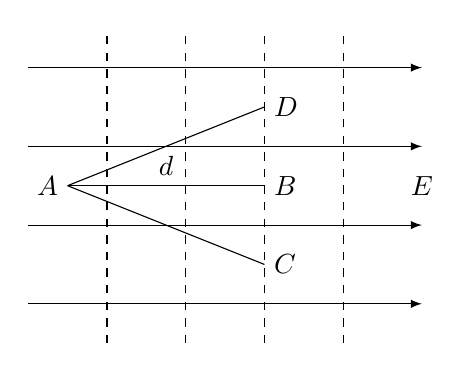
\begin{tikzpicture}[>=latex,scale=1.0]
  % \useasboundingbox(-1,-2)rectangle(8,6);
  \foreach \x in {1,2,3,4}
  {
  \draw[dashed] (\x,.5)--(\x, 4.5);
  \draw[->](0,\x)--(5,\x);
  }
  \node at (5,2.5){$E$};
  \draw (.5,2.5)node [left]{$A$}--node[above]{$d$}(3,2.5)node [right]{$B$};
  \draw (.5,2.5)--(3,3.5)node [right]{$D$};
  \draw (.5,2.5)--(3,1.5)node [right]{$C$};
\end{tikzpicture}
\end{document}